%!TEX root = ../main.tex
%%%%%%%%%%%%%%%%%%%%%%%%%%%%%%%%%%
% Links:
%
% Difficulty: Easy/Medium Companies: 
%%%%%%%%%%%%%%%%%%%%%%%%%%%%%%%%%%

%\chapterimage{header}

\chapter{Power set generation}
\label{ch:power_set}
\section*{Introduction}
The concept of power set is familiar to many because it is a topic of the first
introductory math courses on set theory. 
The problem described in this chapter is about writing
an algorithm that is capable of finding the power set of a given set. 
We will discuss two different approaches: 
\begin{enumerate}
    \item one deriving straightforwardly  from the recursive definition of
    power set\footnote{The power set of an empty set is a set that contains one element only: the empty set itself. For a non-empty set $S$, let $e$ be an
    element of $S$ and $T$ be the original $S$ set minus $e$ (the relative complement $T=S \setminus e$). The power set can
    be then defined as the union of two distinct power sets: 
    \begin{enumerate*}
        \item the power set of $T$,
        \item and the power set of $T$ modified in a such way that $e$ is added to all of its elements.
    \end{enumerate*}
    A more formal definition of power set is shown in Equation \ref{eq:power_set_recursive_definition}:
    \begin{equation}
        \mathcal{P}(S)=\begin{cases} 
    \{\{\}\} & \text{if } S=\{\} \\
    \mathcal{P}\{T\} \bigcup \{t \bigcup \{e\} \: : t \in \mathcal{P}\{T\}\} \text{ where } e \in S, \text{ and } T = P \setminus \{e\} & \text{otherwise}
    \end{cases}
    \label{eq:power_set_recursive_definition}
    \end{equation} 
    } (See Equation \ref{eq:power_set_recursive_definition}),
    \item while the other is based on a clever
    observation about the distribution of the bits in the binary representation of the integers from $0$ to the size of the
    power set. 
\end{enumerate}


\section{Problem statement}
    \begin{exercise}
        Write a function that given a set of elements $S$ returns its power set.
        A power-set of a set $S$ ($\mathcal{P}(S)$) is the set of all its subsets including the empty subset
        ($\emptyset$) and $S$ itself.

        \begin{example}
            \label{ex:power_set:example1}
            \hfill \\
            Given the set $S=\{a,b,c\}$, the following is a correct output for
            this problem: $$\{\{\}, \{a\}, \{b\}, \{c\}, \{a,b\}, \{b,c\}, \{a,c\}, \{a,b,c\} \}$$
        \end{example}
    \end{exercise}

\section{Clarification Questions}

\begin{QandA}
    \item What is the maximum size of the input?
    \begin{answered}
        \textit{The maximum number of element is strictly less than $n < 32$.}
    \end{answered}
    
    \item Are all the elements in the collection distinct?
    \begin{answered}
        \textit{No, the elements are not necessarily distinct. $S$ can contain duplicates.}
    \end{answered}

    \item Can the subset in the power-set appear in any order?
    \begin{answered}
        \textit{Yes, subsets can appear in any order. 
        For example the following is also a valid output for the input shown in Example \ref{ex:power_set:example1}:} 
        $\{\{\}, \{b,c\}, \{a\}, \{a,b\}, \{a,b,c\}, \{b\}, \{a,c\}, \{c\} \}$
    \end{answered}
\end{QandA}

\section{Discussion}
\label{sec:powerset:discussion}
There is one key point that should immediately be noticed: The power set of a collection of
    $n$ elements has size $2^n$. The proof of this fact is relatively easy, and it boils
    down to the fact that a subset of $S$ can be uniquely identified by a list $X=\{x_0,x_1,\ldots x_{|S|}\}$ 
    of $|S|$ binary variables each carrying the information about whether 
    $S_i$ is part of the subset; $x_i$ answers the question: should $S_i$ be part of this subset? if $x_i$ is true the answer is yes, otherwise it is no.
    Because we have two possible choices we can make for every element of $S$ (either
    take it or not), then the total number of the possible subset is: $2 \times 2
    \times \ldots \times 2 = 2^{|P|}$. 
    Two choices for the first element, two for the second, and so
    on until the last element of $P$.
    
    This fact together with the constraint on $|S|$ ($|S| < 32)$ is a strong hint towards the fact
    that an exponential solution is expected.
    After all, we are required to output all the elements
    of the power set, and thus the number of operations of an algorithm designed for this task cannot be less
    than the size of the power set itself. 


\subsection{Backtracking}
The first solution presented in this chapter is based on the fact that  during the generation of
one of the elements of the power set a decision has to be taken for each element of the original
set, on whether to include or not the element into the subset. 
When a decision for the first element is taken, we are left with are $|S|-1$ decisions
before we have created a valid subset of $|S|$.

This kind of process can be easily visualized with a tree (see Figure \ref{ref:power_set_decision_trees}) 
where a node at level $i$
represents a decision for the $i^{th}$ element and a path from the root to a leaf uniquely
identifies a subset of $S$ as, after having traversed all the levels down to a leaf, $n$ decisions have been taken: 
one for each element of $S$. 
All paths from the root to the leaves, represent the power set, and therefore, in
order to solve this problem, we have to visit the entire tree.


A general way to deal with such type of problems is by using backtracking to try all possible
decisions.
The idea is that, for all elements, from first to last, we are going to
explore the two available possibilities: either take or exclude the
it from the subset.
Backtracking is a general technique allowing to enumerate and explore
large search spaces. We can apply it to this problem by making a decision for
the first element and continuing from there to generate all possible subsets
where the first decision is never changed. 
When there are no more subsets to generate, we backtrack and change our first
decisions to the next possible one and repeat the process of generating all possible subsets.

The proposed solution will incrementally construct one subset at a time, 
using an integer variable to keep track of which element we are currently taking the decision for.
The base case of the recursion happens when there is no more decision
to take, meaning that the current subset is ready to be included in the solution (it has been
produced after $n$ decision steps).

The C++ code implementing the idea above is shown in Listing \ref{list:power_set_backtracking}. The complexity of this solution is exponential i.e. $O(2^n)$ which as already pointed out is as good as
it gets.


\lstinputlisting[language=c++, caption="C++ to the power set generation using backtracking",label=list:power_set_backtracking]{sources/power_set/power_set_backtracking.cpp}


\begin{figure}
    \centering
    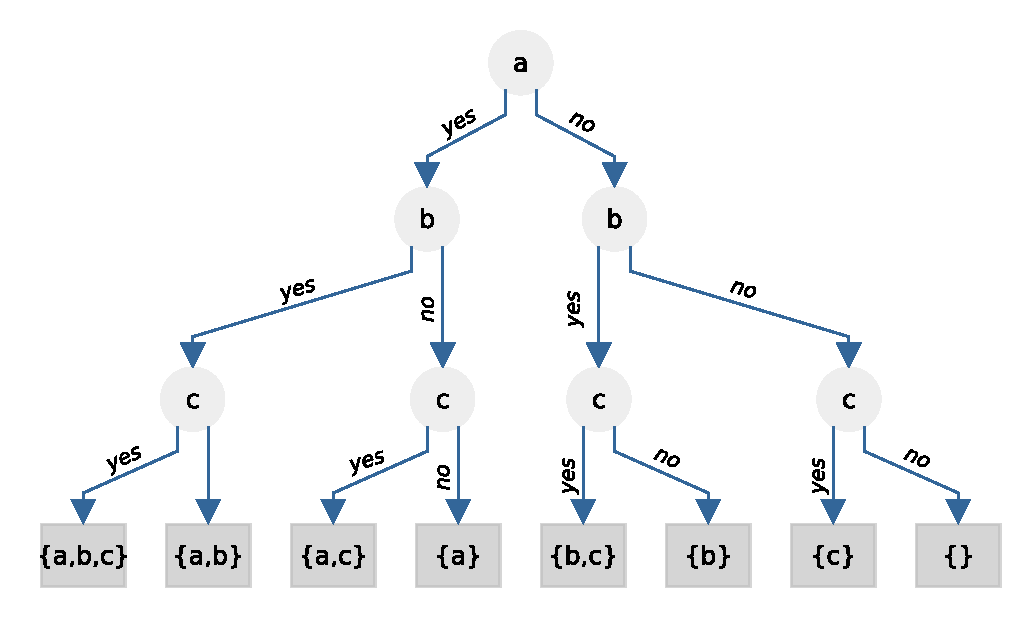
\includegraphics[width=\textwidth]{sources/power_set/images/tree}
    \caption[Decision tree for the power-set generation using backtracking.]{Decision tree for the power-set generation using backtracking. At level $i$ are the decision for the element $i$ in the original set. A labal marked with yes identifies the decision to take the corrensponding element into the subset, while a node labeled with no the opposite. At the last level is the power set.}
    \label{ref:power_set_decision_trees}
\end{figure}

The advantages of using the backtracking framework to solve this problem are that, once we notice
that this problem can be solved by fully exploring the search tree, then we can immediately
start writing the code and rely on our experience as backtracking algorithm writers to implement a correct
solution with the added bonuses of being concise and short when written in a recursive  form (which gives you fewer chances to make mistakes, and less code to debug and explain)  as well
as well understood.
The downside is that the iterative implementation can be a little harder and more verbose to write.
Regardless of which one you choose, the interviewer is going to be pleased with your code provided you get to the final solution
without making too many implementation mistakes (forgetting to add the base case is a pretty common one).
\subsection{Bit Manipulation}
Another approach that can be used to solve this problem is based on the fact that the values of the
bits of the numbers $\{0,1,2,\ldots, s^n-1\}$  already provide all the information necessary to decide whether to include or not an element from the original set into a subset. 
The main idea is that the binary representation of the numbers from $0$ to $2^{n}-1$ is the power-set of $n$ bits.
In other words, the binary representation of any of those numbers can be used to build one subset out
of the $n$ elements of the input set. 

For instance given the input $S=\{a,b,c\}$ the Table \ref{tab:mapping_value_bits} shows numbers from $0$ to $2^3-1 = 8$ and their bit
representation (in the second column) and how such information about which bit is set can be used to construct one
subset of the power-set of $S$ ( in the third column). When the $i^{th}$ bit is set (its value is $1$), it means that
corresponding $i^{th}$ element of $S$ is chosen, while an unset bit (with value $0$) means it is
excluded.

\begin{table}
    \centering
    \begin{tabular}{|l|l|l|}
        \hline
        Value & Bits & Subset\\ \hline
        0     & 000  & $\{\}$\\ \hline
        1     & 001  & $\{c\}$\\ \hline
        2     & 010  & $\{b\}$\\ \hline
        3     & 011  & $\{b,c\}$\\ \hline
        4     & 100  & $\{a\}$\\ \hline
        5     & 101  & $\{a,c\}$\\ \hline
        6     & 110  & $\{a,b\}$\\ \hline
        7     & 111  & $\{a,b,c\}$ \\ \hline
    \end{tabular}
    \caption[Mapping between bits and element of the power set.]{This table shows a 1-to-1 mapping between integer values, their binary representation and an element of the power set.}
    \label{tab:mapping_value_bits}
\end{table}

This idea can be used to write an algorithm in which all the numbers in the range $\{0,1,2,\ldots,
s^n-1\}$ are considered and each of them is used to generate a subset of the final solution.
Every number from such range maps uniquely to a subset of the power set. It is not
surprising when we think about the meaning of a bit in the binary representation of integers. One
can build a number by summing up powers of $2$ and the bits contain the information on whether a
certain power of two should be added to the final value for the represented number or not. With $n$
bits one can represent $2^n$ numbers, each corresponding to one subset of the power set of those
$n$ bits.

Listing \ref{list:power_set_bits} shows  a possible C++ implementation of the idea above
\footnote{Notice the usage of the \texttt{reserve}
function that should be used in all those scenarios when we already know the final size of the
collection we are building. This saves times because avoids intermediate allocation and copy that
must happen during the resize of the vector.}.
The complexity of this implementation is, not
surprisingly, $O(2^n)$. We also pay, in practice a constant price of $32$ for each number we loop through
since we need to inspect all the values of its bits.
The proposed implementation
assumes that the size of \lstinline[columns=fixed]{int} is $4$ bytes, 
which is true for most architecture but not for all\cite{cit::std::fundamentaltypes}. A better
implementation would use \lstinline[columns=fixed]{std::numeric_limits<int>::digits} instead of
the magic number $32$.



\lstinputlisting[language=c++, caption="C++ backtracking solution to the problem of generating the power set.",label=list:power_set_bits]{sources/power_set/power_set_bit_manipulation.cpp}


%\section{Common variations}

%\section{Conclusion}
